\documentclass[titlepage,11pt,a4paper]{article}
\usepackage{booktabs,float,zharticle,indentfirst,listings,xcolor,multirow}
\setmainfont{Adobe Song Std}
\title{
\includegraphics[scale=0.06]{logo.pdf}\\\song 数字设计原理与实践\\课程设计报告}
\author{\song 学生姓名~\makebox[10em][c]{\uline{\hfill \hfill}}\\
	\song 学~~~~~~~~~~号~\makebox[10em][c]{\uline{\hfill \hfill}}\\
	\song 专~~~~~~~~~~业~\makebox[10em][c]{\uline{\hfill \hfill}}\\
	\song 指导教师~\makebox[10em][c]{\uline{\hfill \hfill}}\\
	\song 指导单位~\makebox[10em][c]{\uline{\hfill 电子科技大学\hfill}}}
\date{}
\begin{document}
\maketitle
\begin{CJK}{UTF8}{gbsn}
\begin{abstract}

\CJKindent 本报告主要内容为:使用 Verilog HDL 的三段式状态机设计方法,设计序列检测器。检测序列为110100。
\end{abstract}
\tableofcontents
\section{课程设计概述}{

\CJKindent 本课程设计首先进行状态机设计,然后使用 Verilog HDL 进行状态机描述,然后仿真验证电路并综合出电路,从而进一步熟悉硬件描述语言及其开发环境的使用。其中Verilog文件通过文本编辑软件输入,仿真验证过程使用Icarus Verilog,波形查看使用GTKWave,综合过程用到了Quartus II Web Edition。以上均为免费软件,Free And NO Piracy!
}
\section{课程设计目的}
\begin{enumerate}
	\item 进一步学习 Verilog HDL ,能利用其进行简单的状态机描述及测试平台的设计;
	\item 熟悉 Quartus Ⅱ 的基本操作,通过该软件进行综合;
	\item 学习Iverilog和GTKWave的使用,熟悉基本仿真命令。
	\item 结合实践加深对理论知识的理解。
	\end{enumerate}
\section{课程设计步骤}
\begin{enumerate}
	\item 状态机设计

	\CJKindent 设计序列为110100,采用moore机,使用了7个状态。对于7个状态的状态机,$\lceil \log_{2}7 \rceil=3$,因此该状态机理论上需要3个D触发器。

	\CJKindent Quartus II有状态图输入功能。状态图设计如下:
	\begin{figure}[H]
		\centering
		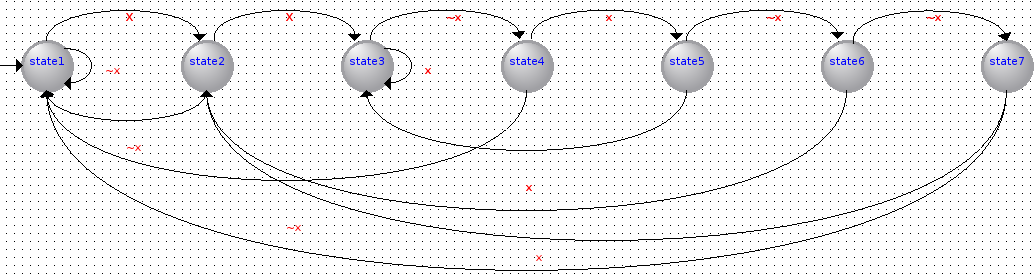
\includegraphics[scale=0.4]{editstate.png}
		\caption{状态图设计}
		\end{figure}

	\CJKindent 根据状态图得到的状态转移输出表:

	\begin{table}[ht]
		\centering
		    \begin{tabular}{*{9}{cccc}}
			        \toprule
				\multirow{2}*{$S$}&\multicolumn{2}{c}{$X$}&\multirow{2}*{$Z$}\\
				\cmidrule(lr){2-3} & 0 &1\\
				    \midrule
				    S1&  S1& S2& 0 \\
				    S2&  S1& S3& 0 \\
				    S3&  S4& S3& 0 \\
				    S4&  S1& S5& 0 \\
				    S5&  S6& S3& 0 \\
				    S6&  S7& S2& 0 \\
				    S7&  S1& S2& 1 \\
				\cmidrule(){2-3} 
				&\multicolumn{2}{c}{$S^*$}\\
				        \bottomrule
					    \end{tabular}
	    \caption{状态/输出表}
    \end{table}

	\item Verilog HDL 程序设计

	\CJKindent 为进一步掌握Verilog HDL,不采用 EDA 软件由状态图生成的 Verilog 程序,而是自行设计 Verilog 程序并用文本编辑软件输入。遵循三段式设计方法,根据状态机写出如下 Verilog 代码:
{\tiny
{\mono
	\begin{lstlisting}[language=Verilog,numbers=left,keywordstyle=\color{blue!70},numberstyle=\tiny,escapechar=`,commentstyle=\color{red!50!green!50!blue!50},frame=shadowbox,rulesepcolor=\color{red!20!green!20!blue!20}]
/*File Name : seqdetector.v
 *Description : The Verilog HDL file of DDPP's project3
 *Author : `\color{red!50!green!50!blue!50}皮文伍`
 *Date : 2014/07/04 18:13'
 *Annotate : moore machine of sequence 110100 detector.
 */

module seqdetector(signalin,signalout,reset_n,clk);

//initialize
input signalin,reset_n,clk;
output signalout;
reg signalout;
reg [2:0] current_state,next_state;

//state assignment
parameter S1=3'b000,S2=3'b001,S3=3'b010,S4=3'b011,S5=3'b100,S6=3'b101,S7=3'b110;

//define reset low level enable
always @(posedge clk,negedge reset_n) //clock rising edge effective
begin
	if(!reset_n)
		current_state<=S1;
	else
		current_state<=next_state;
end

//detect sequence 110100
always @ *
begin
	case (current_state)
		S1:begin
			if(signalin) next_state=S2;
			else next_state=S1;
		end
		S2:begin
			if(signalin) next_state=S3;
			else next_state=S1;
		end
		S3:begin
			if(~signalin) next_state=S4;
			else next_state=S3;
		end
		S4:begin
			if(signalin) next_state=S5;
			else next_state=S1;
		end
		S5:begin
			if(~signalin) next_state=S6;
			else next_state=S3;
		end
		S6:begin
			if(~signalin) next_state=S7;
			else next_state=S2;
		end
		S7:begin
			if(signalin) next_state=S2;
			else next_state=S1;
		end
	endcase
end

//define output of each states
always @(posedge clk,negedge reset_n)
begin
	if(!reset_n)
		signalout<=0;
	else
		case(current_state)
			S1:signalout<=0;
			S2:signalout<=0;
			S3:signalout<=0;
			S4:signalout<=0;
			S5:signalout<=0;
			S6:signalout<=0;
			S7:signalout<=1;
		endcase
end

endmodule

\end{lstlisting}
}}
	\item Verilog 仿真验证

		编译成功后设计 testbench,产生激励信号,进行功能仿真,验证输出是否正确。
		
		以下是testbench:
{\tiny
{\mono
	\begin{lstlisting}[language=Verilog,numbers=left,keywordstyle=\color{blue!70},numberstyle=\tiny,,commentstyle=\color{red!50!green!50!blue!50},frame=shadowbox,rulesepcolor=\color{red!20!green!20!blue!20}]
`timescale 1ns/1ns
module seqdetector_tb;

	//input signal
	reg x;
	reg rst_n;

	//CLOCK signal
	reg CLK;

	//output
	wire z;

	//Instantiate the module seqdetector
	seqdetector u1(
		.signalout(z),
		.signalin(x),
		.reset_n(rst_n),
		.clk(CLK)
	);
	
	//produce test sequential signal
	always #1 CLK=~CLK;
	initial 
	begin
		CLK=0;
		rst_n=1;
		x=0;
		#1 rst_n=0;
		#1 rst_n=1;

		#2 x=1;
		#2 x=1;
		#2 x=0;
		#2 x=1;
		#2 x=0;
		#2 x=0;
		#2 x=0;
		#2 x=1;
		#2 x=1;
		#2 x=0;
		#2 x=1;
		#2 x=1;
		#2 x=0;
		#2 x=1;
		#2 x=0;
		#2 x=0;
		#2 x=0;
		#2 x=0;
		#2 \$finish;
	end

	//create vcd file for watching waveform diagram.
	initial
	begin
		\$dumpfile("seqdetector_tb.vcd");
		\$dumpvars;
	end
endmodule
\end{lstlisting}
}}

\CJKindent 使用 Icarus Verilog进 行仿真,输出波形文件seqdetector\_tb.vcd,以下是是GTKWave查看的波形图:
	\begin{figure}[H]
		\centering
		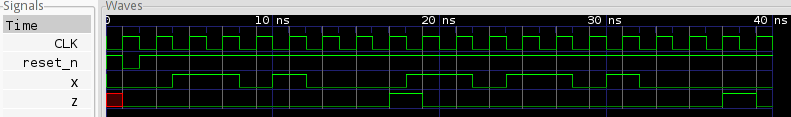
\includegraphics[width=13cm,height=3cm]{waveform.png}
		\caption{Icarus Verilog 仿真波形图}
		\end{figure}

	\CJKindent 状态机设计为上升沿触发。从图中可以看到,当输入端x检测到110100序列后,输出端z输出高电平,与所需功能相符合。从图中还可以看出输出信号有一个时钟周期的延迟,这是moore机的典型特点。
	
	\item 仿真验证功能后使用Quartus II综合

	使用Quartus II综合出的RTL电路图:
	\begin{figure}[H]
		\centering
		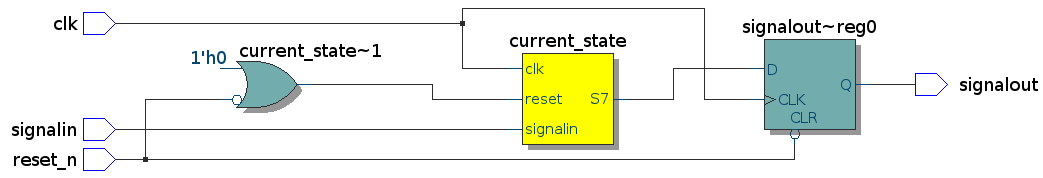
\includegraphics[scale=0.3]{RTLdiagram.png}
		\caption{Quartus II综合RTL电路图}
		\end{figure}
		
	使用Quartus II综合出的状态图:
	\begin{figure}[H]
		\centering
		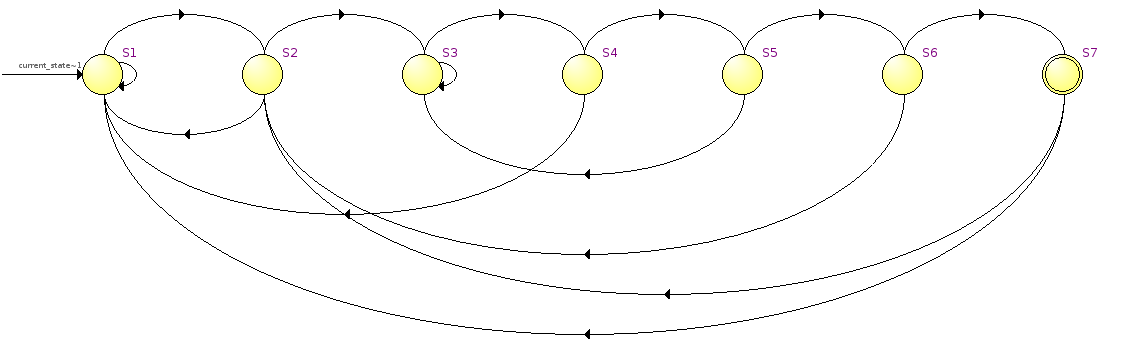
\includegraphics[scale=0.3]{generatestate.png}
		\caption{Quartus II综合状态图}
		\end{figure}
		与起初手工设计的状态图比较,Verilog HDL 描述所综合出的状态图完全一样,证明 Verilog 程序实现了110100序列检测器的功能!
\end{enumerate}
\end{CJK}
\end{document}
